
    Since a DSM describes a square adjacency matrix, it can be represented in an equivalent directed graph where nodes represent analysis tools and
    edges represent information exchange between those tools. An alternate matrix based syntax, called a
    Functional Dependence Table (FDT), was proposed by Michelena and Papalambros.
    FDT represents the relationship between functions, including objectives and constraints, and their values\cite{Michelena1997}. Similar to DSM
    FDT also describes an adjacency matrix of a graph. Unlike the DSM graph, however, a FDT graph is an undirected
    graph where nodes can represent analysis tools, objectives, or constraints. Edges between nodes represent a dependence on the same
    variable value. By searching the FDT graph for clusters of totally connected nodes Wagner and Papalambros were identify groups of
    analysis tools that were all dependent on the same input variables and used that to make partitioning decisions \cite{Wagner1993}.

    It is possible to combine the syntax of an FDT and a DSM by making a subtle extension to a traditional DSM specification. Normally, a DSM is given
    with analysis tools as nodes and variable dependencies given as edges. Lamb and Martins included the variables, objectives, and constraint functions
    as nodes in an Extented DSM (XDSM)\cite{Lambe2012} in order to capture a more complete problem formulation for MDAO problems. With XDSM
    it is possible to also encompass the relationships defined in an FDT. Figure \ref{fig:dsm_full}
    illustrates the same notional analysis as in Figure \ref{fig:dsm_simple} represented as an XDSM.
    The dashed boxes indicate groups of nodes that could be collapsed back down to retrieve the simpler
    DSM from above. Beyond specifying relationships between data in a problem formulation, XDSM also includes syntax to describe the
    procedural order of any given solution path. Figure \ref{fig:xdsm_full} shows the full XDSM specification for solving the notional
    analysis with a traditional Multidisciplinary Design Feasible (MDF) architecture.

    \begin{figure}[!hbp]
        \begin{center}
        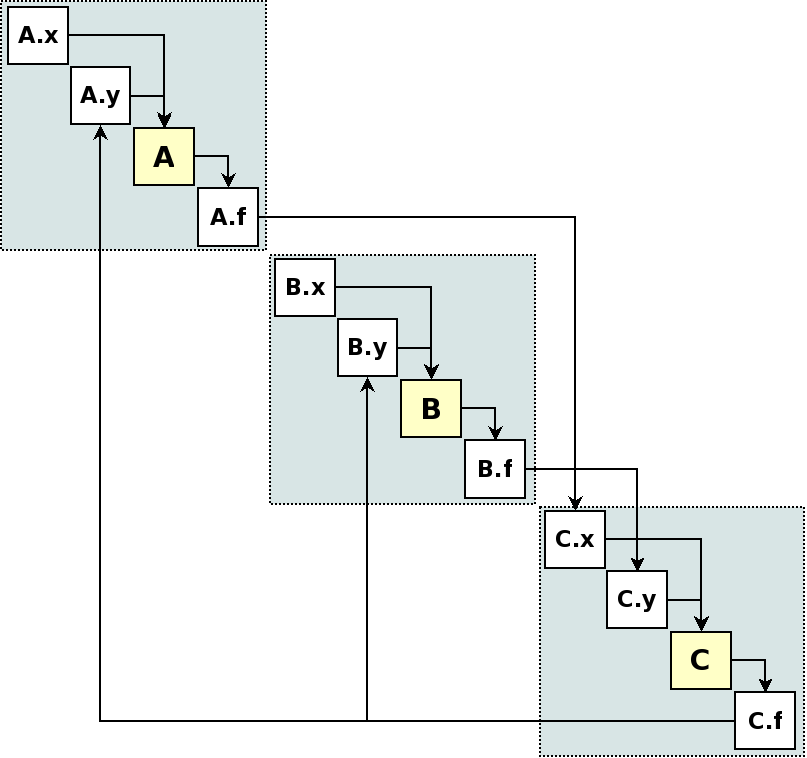
\includegraphics[width=.75\textwidth]{images/dsm_full}
        \caption{Extended DSM graph for a notional analysis \label{fig:dsm_full}}
        \end{center}
    \end{figure}

    
\section{Graph Based Problem Formulation Syntax}
    \subsection{Formulation Graph Syntax}
    Rather than start with an adjacency, we chose to work directly with a directed cyclic graph to develop a syntax for the FPF. 
    The following information must be provided to start:
    \begin{itemize}
        \item Analysis blocks: an analysis block represents any calculation, and each comes with
            \begin{itemize}
                \item local inputs
                \item local outputs 
                \item execution properties: the properties associated with running the code, such as run time.
            \end{itemize}
        \item Global parameters: these may serve as fixed inputs to the local inputs of analysis blocks
        \item Global outputs: these may represent
            \begin{itemize}
                \item objectives
                \item constraints
                \item residuals: (not sure)
            \end{itemize}
    \end{itemize}

    The graph representation of a data flow is cast to utilize the extensive library of algorithms in graph theory to analyze a directed weighted graph. 
    Edge weights are used to represent the metrics associated with a data flow
    \begin{itemize}
        \item Run time: this metric is a property of an analysis block
        \item Fidelity: this metric is a property of an individual local output
        \item Expected Convergence
    \end{itemize}

    The key assumption is that identical variables are recognized as such. This serves as the basis for creating a data flow by connecting compatible input and output nodes with a directed edge. 
    In order to represent the fact that execution of an analysis code does not depend on the number of outputs being used, it is represented as depicted in the following figure (not made yet).
    
    This information immediately leads to the maximal connectivity graph, which is formed by placing a directed edge from each local output or global parameter to each matching local input or global output. 
    Whenever multiple edges are connected to a single input a conflict occurs because only one may be used. Resolving these conflicts is one key challenge in creating a data flow.
%    \begin{itemize}
%        \item Specify analyses
%        \item Connections between analyses 
%            \begin{itemize}
%                \item local variables
%                \item global variables? Use "fake" node that broadcasts out to the rest of the graph? 
%            \end{itemize}
%        \item Cycles indicate coupling
%        \item Cycles for design variables->objectives/constraints
%        \item Objectives/constraints are just outputs? Special nodes? 
%        \item Residuals are just outputs? Special nodes? 
%        \item Parameters are just input nodes that are not design variables (use identifies these)
%        \item FPF no solvers/optimizers anywhere in it
%    \end{itemize}

    \subsection{Solution Graph Syntax}
    What is the difference between a problem formulation and a problem solution method? Convert from a cyclic graph, to an acyclic graph
    \begin{itemize}
        \item cycles indicate convergence loops or design varaible loops
        \item Problem can't be solved until all loops are *removed* by adding in solvers/optimizers
        \item *special* nodes for solvers and optimizers that *break* loops (from an algorithmic point of view)
        \item FPF represents the minimal amount of information necessary to define a problem
        \item Any solution path grows the graph complexity by adding edges and nodes (or possibly have an empty solution graph, which you build up
        as you remove edges from problem formulation graph?)
    \end{itemize}

    
\section{Example Problem}

\section{Applications}

\section{Conclusions}

\bibliography{library}
\end{document}